\section{Shared task on word sense induction}

\subsection{}

\begin{frame}{A shared task on WSI}
  
  \begin{itemize}
  \item An \textbf{\alert{ACL SIGSLAV}} sponsored shared task on \textbf{word sense induction} (WSI) for the Russian language.
 \end{itemize} 
  
  \begin{itemize}
    \item \textbf{More details}: \url{http://russe.nlpub.org/2018/wsi}
     
  \end{itemize}
  
  \begin{center}
  	
\includegraphics[width=0.2\textwidth]{figures/acl}
  \end{center}
  
   \begin{center}
  	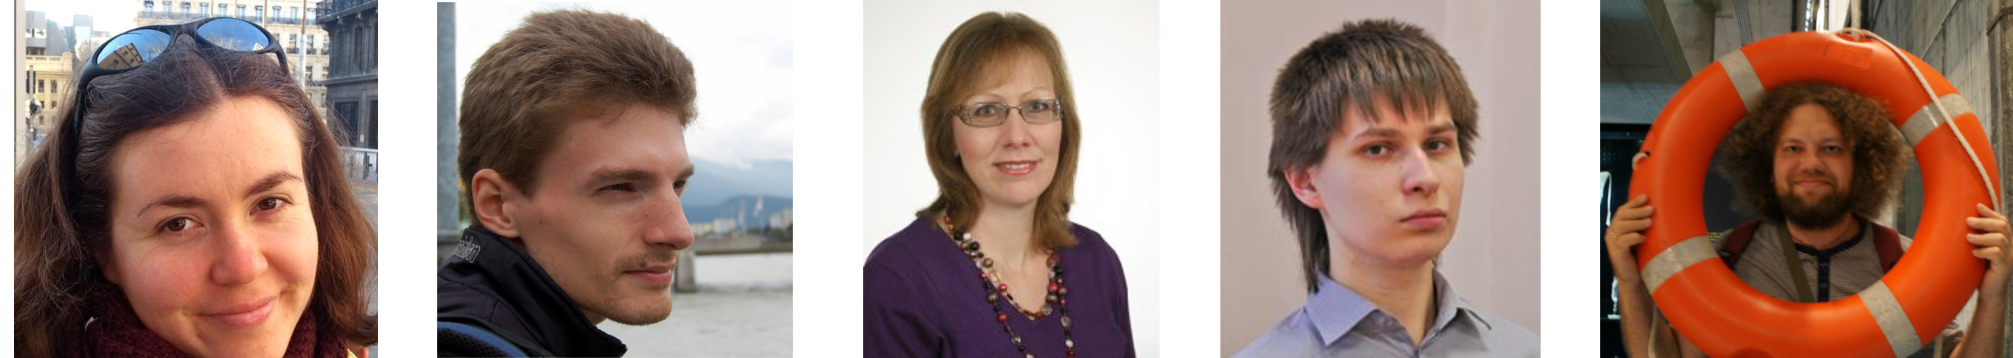
\includegraphics[width=0.99\textwidth]{figures/russe-team}
  \end{center}
\end{frame}



\begin{frame}{A lexical sample WSI task}
  
  \begin{itemize}
  	\item \textbf{Target word}, e.g. ``bank''.
  	
  	\pause 
  	
  	\item \textbf{Contexts} where the word occurs, e.g.: 
  	\begin{itemize}
  	\item ``river \textbf{bank} is a slope beside a body of water''
  	\item ``\textbf{bank} is a financial institution that accepts deposits''
  	\item ``Oh, the \textbf{bank} was robbed. They took about a million dollars.''
  	\item ``\textbf{bank} of Elbe is a good and popular hangout spot complete with good food and fun''
  	\end{itemize}
  	
  	\pause 
  	
  	\item You need to \textbf{{group} the contexts by senses}:
  	\begin{itemize}
  	\item \textcolor{Cerulean}{``river \textbf{bank} is a slope beside a body of water''}
  	\item \textcolor{Cerulean}{``\textbf{bank} of Elbe is a good and popular hangout spot complete with good food and fun''}
  	\item \alert{``\textbf{bank} is a financial institution that accepts deposits''}
  	\item \alert{``Oh, the \textbf{bank} was robbed. They took about a million dollars.''}
  	\end{itemize}
  	 
  \end{itemize}
  
\end{frame}

